% Options for packages loaded elsewhere
\PassOptionsToPackage{unicode}{hyperref}
\PassOptionsToPackage{hyphens}{url}
\PassOptionsToPackage{dvipsnames,svgnames,x11names}{xcolor}
%
\documentclass[
  letterpaper,
  DIV=11,
  numbers=noendperiod]{scrreprt}

\usepackage{amsmath,amssymb}
\usepackage{iftex}
\ifPDFTeX
  \usepackage[T1]{fontenc}
  \usepackage[utf8]{inputenc}
  \usepackage{textcomp} % provide euro and other symbols
\else % if luatex or xetex
  \usepackage{unicode-math}
  \defaultfontfeatures{Scale=MatchLowercase}
  \defaultfontfeatures[\rmfamily]{Ligatures=TeX,Scale=1}
\fi
\usepackage{lmodern}
\ifPDFTeX\else  
    % xetex/luatex font selection
  \setmainfont[]{TeX Gyre Termes X}
  \setsansfont[]{TeX Gyre Heros}
  \setmonofont[]{TeX Gyre Cursor}
  \setmathfont[]{TeX Gyre Termes Math}
\fi
% Use upquote if available, for straight quotes in verbatim environments
\IfFileExists{upquote.sty}{\usepackage{upquote}}{}
\IfFileExists{microtype.sty}{% use microtype if available
  \usepackage[]{microtype}
  \UseMicrotypeSet[protrusion]{basicmath} % disable protrusion for tt fonts
}{}
\makeatletter
\@ifundefined{KOMAClassName}{% if non-KOMA class
  \IfFileExists{parskip.sty}{%
    \usepackage{parskip}
  }{% else
    \setlength{\parindent}{0pt}
    \setlength{\parskip}{6pt plus 2pt minus 1pt}}
}{% if KOMA class
  \KOMAoptions{parskip=half}}
\makeatother
\usepackage{xcolor}
\setlength{\emergencystretch}{3em} % prevent overfull lines
\setcounter{secnumdepth}{5}
% Make \paragraph and \subparagraph free-standing
\ifx\paragraph\undefined\else
  \let\oldparagraph\paragraph
  \renewcommand{\paragraph}[1]{\oldparagraph{#1}\mbox{}}
\fi
\ifx\subparagraph\undefined\else
  \let\oldsubparagraph\subparagraph
  \renewcommand{\subparagraph}[1]{\oldsubparagraph{#1}\mbox{}}
\fi

\usepackage{color}
\usepackage{fancyvrb}
\newcommand{\VerbBar}{|}
\newcommand{\VERB}{\Verb[commandchars=\\\{\}]}
\DefineVerbatimEnvironment{Highlighting}{Verbatim}{commandchars=\\\{\}}
% Add ',fontsize=\small' for more characters per line
\usepackage{framed}
\definecolor{shadecolor}{RGB}{241,243,245}
\newenvironment{Shaded}{\begin{snugshade}}{\end{snugshade}}
\newcommand{\AlertTok}[1]{\textcolor[rgb]{0.68,0.00,0.00}{#1}}
\newcommand{\AnnotationTok}[1]{\textcolor[rgb]{0.37,0.37,0.37}{#1}}
\newcommand{\AttributeTok}[1]{\textcolor[rgb]{0.40,0.45,0.13}{#1}}
\newcommand{\BaseNTok}[1]{\textcolor[rgb]{0.68,0.00,0.00}{#1}}
\newcommand{\BuiltInTok}[1]{\textcolor[rgb]{0.00,0.23,0.31}{#1}}
\newcommand{\CharTok}[1]{\textcolor[rgb]{0.13,0.47,0.30}{#1}}
\newcommand{\CommentTok}[1]{\textcolor[rgb]{0.37,0.37,0.37}{#1}}
\newcommand{\CommentVarTok}[1]{\textcolor[rgb]{0.37,0.37,0.37}{\textit{#1}}}
\newcommand{\ConstantTok}[1]{\textcolor[rgb]{0.56,0.35,0.01}{#1}}
\newcommand{\ControlFlowTok}[1]{\textcolor[rgb]{0.00,0.23,0.31}{#1}}
\newcommand{\DataTypeTok}[1]{\textcolor[rgb]{0.68,0.00,0.00}{#1}}
\newcommand{\DecValTok}[1]{\textcolor[rgb]{0.68,0.00,0.00}{#1}}
\newcommand{\DocumentationTok}[1]{\textcolor[rgb]{0.37,0.37,0.37}{\textit{#1}}}
\newcommand{\ErrorTok}[1]{\textcolor[rgb]{0.68,0.00,0.00}{#1}}
\newcommand{\ExtensionTok}[1]{\textcolor[rgb]{0.00,0.23,0.31}{#1}}
\newcommand{\FloatTok}[1]{\textcolor[rgb]{0.68,0.00,0.00}{#1}}
\newcommand{\FunctionTok}[1]{\textcolor[rgb]{0.28,0.35,0.67}{#1}}
\newcommand{\ImportTok}[1]{\textcolor[rgb]{0.00,0.46,0.62}{#1}}
\newcommand{\InformationTok}[1]{\textcolor[rgb]{0.37,0.37,0.37}{#1}}
\newcommand{\KeywordTok}[1]{\textcolor[rgb]{0.00,0.23,0.31}{#1}}
\newcommand{\NormalTok}[1]{\textcolor[rgb]{0.00,0.23,0.31}{#1}}
\newcommand{\OperatorTok}[1]{\textcolor[rgb]{0.37,0.37,0.37}{#1}}
\newcommand{\OtherTok}[1]{\textcolor[rgb]{0.00,0.23,0.31}{#1}}
\newcommand{\PreprocessorTok}[1]{\textcolor[rgb]{0.68,0.00,0.00}{#1}}
\newcommand{\RegionMarkerTok}[1]{\textcolor[rgb]{0.00,0.23,0.31}{#1}}
\newcommand{\SpecialCharTok}[1]{\textcolor[rgb]{0.37,0.37,0.37}{#1}}
\newcommand{\SpecialStringTok}[1]{\textcolor[rgb]{0.13,0.47,0.30}{#1}}
\newcommand{\StringTok}[1]{\textcolor[rgb]{0.13,0.47,0.30}{#1}}
\newcommand{\VariableTok}[1]{\textcolor[rgb]{0.07,0.07,0.07}{#1}}
\newcommand{\VerbatimStringTok}[1]{\textcolor[rgb]{0.13,0.47,0.30}{#1}}
\newcommand{\WarningTok}[1]{\textcolor[rgb]{0.37,0.37,0.37}{\textit{#1}}}

\providecommand{\tightlist}{%
  \setlength{\itemsep}{0pt}\setlength{\parskip}{0pt}}\usepackage{longtable,booktabs,array}
\usepackage{calc} % for calculating minipage widths
% Correct order of tables after \paragraph or \subparagraph
\usepackage{etoolbox}
\makeatletter
\patchcmd\longtable{\par}{\if@noskipsec\mbox{}\fi\par}{}{}
\makeatother
% Allow footnotes in longtable head/foot
\IfFileExists{footnotehyper.sty}{\usepackage{footnotehyper}}{\usepackage{footnote}}
\makesavenoteenv{longtable}
\usepackage{graphicx}
\makeatletter
\def\maxwidth{\ifdim\Gin@nat@width>\linewidth\linewidth\else\Gin@nat@width\fi}
\def\maxheight{\ifdim\Gin@nat@height>\textheight\textheight\else\Gin@nat@height\fi}
\makeatother
% Scale images if necessary, so that they will not overflow the page
% margins by default, and it is still possible to overwrite the defaults
% using explicit options in \includegraphics[width, height, ...]{}
\setkeys{Gin}{width=\maxwidth,height=\maxheight,keepaspectratio}
% Set default figure placement to htbp
\makeatletter
\def\fps@figure{htbp}
\makeatother
\newlength{\cslhangindent}
\setlength{\cslhangindent}{1.5em}
\newlength{\csllabelwidth}
\setlength{\csllabelwidth}{3em}
\newlength{\cslentryspacingunit} % times entry-spacing
\setlength{\cslentryspacingunit}{\parskip}
\newenvironment{CSLReferences}[2] % #1 hanging-ident, #2 entry spacing
 {% don't indent paragraphs
  \setlength{\parindent}{0pt}
  % turn on hanging indent if param 1 is 1
  \ifodd #1
  \let\oldpar\par
  \def\par{\hangindent=\cslhangindent\oldpar}
  \fi
  % set entry spacing
  \setlength{\parskip}{#2\cslentryspacingunit}
 }%
 {}
\usepackage{calc}
\newcommand{\CSLBlock}[1]{#1\hfill\break}
\newcommand{\CSLLeftMargin}[1]{\parbox[t]{\csllabelwidth}{#1}}
\newcommand{\CSLRightInline}[1]{\parbox[t]{\linewidth - \csllabelwidth}{#1}\break}
\newcommand{\CSLIndent}[1]{\hspace{\cslhangindent}#1}

\newcommand{\C}{{\mathbb{{C}}}}
\newcommand{\R}{{\mathbb{{R}}}}
\newcommand{\Q}{{\mathbb{{Q}}}}
\newcommand{\Z}{{\mathbb{{Z}}}}
\newcommand{\N}{{\mathbb{{N}}}}

\newcommand{\uu}[1]{{\symbf{{#1}}}}
\newcommand{\uuuu}[1]{{\symbb{{#1}}}}
\newcommand{\uv}[1]{{\underline{{#1}}}}
\newcommand{\ve}[1]{{\uv{{e}}_{{#1}}}}
\newcommand{\x}{{\uv{{x}}}}
\newcommand{\n}{{\uv{{n}}}}
\newcommand{\eps}{{\uu{{\varepsilon}}}}
\newcommand{\E}{{\uu{{E}}}}
\newcommand{\sig}{{\uu{{\sigma}}}}
\newcommand{\Sig}{{\uu{{\Sigma}}}}
\newcommand{\cod}{{\uv{{\symscr{b}}}}}
\newcommand{\trans}[1]{{{}^{t}{#1}}}
\newcommand{\sotimes}{{\stackrel{s}{\otimes}}}
\newcommand{\sboxtimes}{\stackrel{s}{\boxtimes}}
\newcommand{\norm}[1]{{\lVert{{#1}}\rVert}}
\newcommand{\ud}{{\,\mathrm{d}}}
\DeclareMathOperator{\arcosh}{arcosh}
\DeclareMathOperator{\divz}{div}
\DeclareMathOperator{\divu}{\uv{div}}
\DeclareMathOperator{\hess}{hess}
\DeclareMathOperator{\gradu}{\uv{grad}}
\DeclareMathOperator{\graduu}{\uu{grad}}
\DeclareMathOperator{\Mat}{Mat}
\DeclareMathOperator{\tr}{tr}
\DeclareMathOperator{\ISO}{ISO}

\newcommand{\jump}[1]{[\hspace*{-.15em}[\hspace*{.1em}{#1}%
     \hspace*{.1em}]\hspace*{-.15em}]}
     
\KOMAoption{captions}{tablesignature}
\makeatletter
\@ifpackageloaded{tcolorbox}{}{\usepackage[skins,breakable]{tcolorbox}}
\@ifpackageloaded{fontawesome5}{}{\usepackage{fontawesome5}}
\definecolor{quarto-callout-color}{HTML}{909090}
\definecolor{quarto-callout-note-color}{HTML}{0758E5}
\definecolor{quarto-callout-important-color}{HTML}{CC1914}
\definecolor{quarto-callout-warning-color}{HTML}{EB9113}
\definecolor{quarto-callout-tip-color}{HTML}{00A047}
\definecolor{quarto-callout-caution-color}{HTML}{FC5300}
\definecolor{quarto-callout-color-frame}{HTML}{acacac}
\definecolor{quarto-callout-note-color-frame}{HTML}{4582ec}
\definecolor{quarto-callout-important-color-frame}{HTML}{d9534f}
\definecolor{quarto-callout-warning-color-frame}{HTML}{f0ad4e}
\definecolor{quarto-callout-tip-color-frame}{HTML}{02b875}
\definecolor{quarto-callout-caution-color-frame}{HTML}{fd7e14}
\makeatother
\makeatletter
\makeatother
\makeatletter
\@ifpackageloaded{bookmark}{}{\usepackage{bookmark}}
\makeatother
\makeatletter
\@ifpackageloaded{caption}{}{\usepackage{caption}}
\AtBeginDocument{%
\ifdefined\contentsname
  \renewcommand*\contentsname{Table of contents}
\else
  \newcommand\contentsname{Table of contents}
\fi
\ifdefined\listfigurename
  \renewcommand*\listfigurename{List of Figures}
\else
  \newcommand\listfigurename{List of Figures}
\fi
\ifdefined\listtablename
  \renewcommand*\listtablename{List of Tables}
\else
  \newcommand\listtablename{List of Tables}
\fi
\ifdefined\figurename
  \renewcommand*\figurename{Fig.}
\else
  \newcommand\figurename{Fig.}
\fi
\ifdefined\tablename
  \renewcommand*\tablename{Tab.}
\else
  \newcommand\tablename{Tab.}
\fi
}
\@ifpackageloaded{float}{}{\usepackage{float}}
\floatstyle{ruled}
\@ifundefined{c@chapter}{\newfloat{codelisting}{h}{lop}}{\newfloat{codelisting}{h}{lop}[chapter]}
\floatname{codelisting}{Listing}
\newcommand*\listoflistings{\listof{codelisting}{List of Listings}}
\makeatother
\makeatletter
\@ifpackageloaded{caption}{}{\usepackage{caption}}
\@ifpackageloaded{subcaption}{}{\usepackage{subcaption}}
\makeatother
\makeatletter
\@ifpackageloaded{tcolorbox}{}{\usepackage[skins,breakable]{tcolorbox}}
\makeatother
\makeatletter
\@ifundefined{shadecolor}{\definecolor{shadecolor}{rgb}{.97, .97, .97}}
\makeatother
\makeatletter
\makeatother
\makeatletter
\makeatother
\ifLuaTeX
  \usepackage{selnolig}  % disable illegal ligatures
\fi
\IfFileExists{bookmark.sty}{\usepackage{bookmark}}{\usepackage{hyperref}}
\IfFileExists{xurl.sty}{\usepackage{xurl}}{} % add URL line breaks if available
\urlstyle{same} % disable monospaced font for URLs
\hypersetup{
  pdftitle={Echoes},
  pdfauthor={Jean-François Barthélémy},
  colorlinks=true,
  linkcolor={blue},
  filecolor={Maroon},
  citecolor={Blue},
  urlcolor={Blue},
  pdfcreator={LaTeX via pandoc}}

\title{Echoes}
\usepackage{etoolbox}
\makeatletter
\providecommand{\subtitle}[1]{% add subtitle to \maketitle
  \apptocmd{\@title}{\par {\large #1 \par}}{}{}
}
\makeatother
\subtitle{Extended Calculator of HOmogEnization Schemes}
\author{Jean-François Barthélémy}
\date{2023-09-28}

\begin{document}
\maketitle
\ifdefined\Shaded\renewenvironment{Shaded}{\begin{tcolorbox}[interior hidden, borderline west={3pt}{0pt}{shadecolor}, boxrule=0pt, frame hidden, enhanced, breakable, sharp corners]}{\end{tcolorbox}}\fi

\renewcommand*\contentsname{Table of contents}
{
\hypersetup{linkcolor=}
\setcounter{tocdepth}{2}
\tableofcontents
}
\bookmarksetup{startatroot}

\hypertarget{sec-welcome}{%
\chapter*{Welcome}\label{sec-welcome}}
\addcontentsline{toc}{chapter}{Welcome}

\markboth{Welcome}{Welcome}

\begin{figure}

{\centering 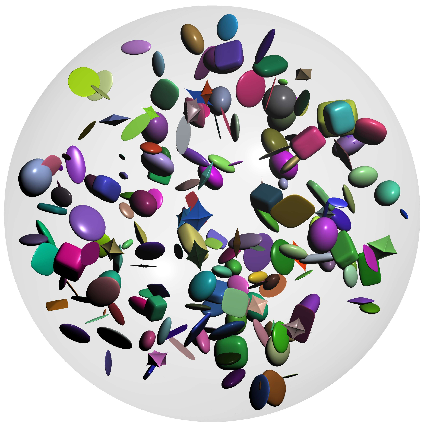
\includegraphics[width=0.4\textwidth,height=\textheight]{images/cover.pdf}

}

\end{figure}

The library \textbf{Echoes} allows to implement various homogenization
schemes involving different types of heterogeneities in the framework of
elasticity, conductivity, viscoelasticity as well as tools to properly
calculate the derivatives of macroscopic stiffness with respect to lower
scale moduli (fundamental tool of the modified secant method in
nonlinear homogenization).

This manual aims at recalling some fundamental aspects of the theory of
homogenization of random media along with a presentation of the main
features of the library \textbf{Echoes} as well as code examples.

\hypertarget{download}{%
\section*{Download}\label{download}}
\addcontentsline{toc}{section}{Download}

\markright{Download}

The core of \textbf{Echoes} has been developed in C++ and wrapped by a
Python interface. Hence its use requires first the installation of a
Python environment with \texttt{pip} executable (for instance
\href{https://www.anaconda.com/products/distribution}{Anaconda}).

Wheel packages can be downloaded for Python 3.7, 3.8 and 3.9 under
Windows or Linux by choosing the appropriate file for your configuration
under the link

https://doi.org/10.5281/zenodo.7348759

Once in possession of the relevant \texttt{.whl} file, the package can
be installed in a console (Anaconda console or any console allowing to
run \texttt{pip}) by

\begin{Shaded}
\begin{Highlighting}[]
\NormalTok{pip install }\OperatorTok{{-}}\NormalTok{U echoes}\OperatorTok{{-}}\NormalTok{XYZ.whl }\CommentTok{\# replacing echoes{-}XYZ.whl by the correct path to the whl file}
\end{Highlighting}
\end{Shaded}

\hypertarget{citation}{%
\section*{Citation}\label{citation}}
\addcontentsline{toc}{section}{Citation}

\markright{Citation}

If you use \textbf{Echoes}, please cite it as
(\protect\hyperlink{ref-echoes}{Barthélémy, Jean-François, 2022})

or in \texttt{bibtex} style

\begin{verbatim}
@misc{Echoes,
 author  = {Barthélémy, Jean-François},
 title   = {Echoes library (Extended Calculator of HOmogEnization Schemes)},
 url     = {https://jfbarthelemy.github.io/echoes/},
 doi     = {10.5281/zenodo.7348759}
 version = {v1.0.0},
 year    = {2022},
 month   = {11}
}
\end{verbatim}

\(\,\)

\bookmarksetup{startatroot}

\hypertarget{sec-intro}{%
\chapter*{Introduction}\label{sec-intro}}
\addcontentsline{toc}{chapter}{Introduction}

\markboth{Introduction}{Introduction}

This book does not provide an exhaustive presentation of the theory of
random medium homogenization (see
(\protect\hyperlink{ref-milton2002}{Milton, 2002}),
(\protect\hyperlink{ref-torquato2002}{Torquato, 2002}) or
(\protect\hyperlink{ref-kachanov2018}{Kachanov and Sevostianov, 2018})
among others) but it is rather intended to recall some of the basic
notations and results related to the implementation of the
\textbf{Echoes} library.

In this manual, some snippets of Python codes calling \textbf{Echoes}
library are presented. Except when it is necessary to show the imported
libraries, the following starting lines will be implicit

\begin{Shaded}
\begin{Highlighting}[]
\ImportTok{import}\NormalTok{ numpy }\ImportTok{as}\NormalTok{ np}
\ImportTok{from}\NormalTok{ echoes }\ImportTok{import} \OperatorTok{*}
\ImportTok{import}\NormalTok{ matplotlib.pyplot }\ImportTok{as}\NormalTok{ plt}
\end{Highlighting}
\end{Shaded}

\(\,\)

\part{Linear elasticity}

\(\,\)

\hypertarget{sec-basics_elas}{%
\chapter{Basic problem of elasticity
homogenization}\label{sec-basics_elas}}

\hypertarget{sec-basics_elas_sys_eq}{%
\section{System of equations}\label{sec-basics_elas_sys_eq}}

Consider a representative volume element (RVE) \(\Omega\) composed of a
heterogeneous material. Neglecting body forces in a problem posed at the
scale of a RVE is consistent with the fact that the order of magnitude
of mechanical effects induced by body forces is in general much lower
than that of the macroscopic strain \(\E\) or stress \(\Sig\) effects
accounting for interactions with particles surrounding the RVE (see
(\protect\hyperlink{ref-dormieux2006}{Dormieux et al., 2006})). The
hypothesis of quasi-static equilibrium is also invoked here to write the
balance law involving the Cauchy stress field \(\sig\)
\begin{equation}\protect\hypertarget{eq-divsigma}{}{
\divu{\sig}=\uv{0} \quad(\Omega)
}\label{eq-divsigma}\end{equation}

In the sequel, the small perturbation hypothesis is adopted so that the
strain field \(\eps\) derives from the displacement one \(\uv{u}\) as
the symmetrical part of its gradient
\begin{equation}\protect\hypertarget{eq-epsgradu}{}{
\eps=\frac{\graduu{\uv{u}}+\trans{\graduu{\uv{u}}}}{2} \quad(\Omega)
}\label{eq-epsgradu}\end{equation}

In the framework of random media homogenization, two types of conditions
applied at the boundary \(\partial\Omega\) of a RVE \(\Omega\) are
usually considered:

\begin{itemize}
\item
  \emph{homogeneous strain boundary conditions} corresponding to
  prescribed displacements \(\uv{u}^g\) at \(\partial\Omega\)
  \begin{equation}\protect\hypertarget{eq-homstrainBC}{}{
  \uv{u}^g=\E\cdot\x \quad(\partial\Omega)
  }\label{eq-homstrainBC}\end{equation} It is noticeable that in this
  case the divergence theorem implies the following relationship between
  the microscopic and macroscopic strain tensors
  \begin{equation}\protect\hypertarget{eq-EhomstrainBC}{}{
  <\eps>_{\Omega}=\frac{1}{\lvert \Omega \rvert}\int_\Omega \eps\ud \Omega
  =\frac{1}{\lvert \Omega \rvert}\int_{\partial\Omega} \uv{u}\sotimes\n \ud S
  =\E
  }\label{eq-EhomstrainBC}\end{equation} where the spatial average over
  a domain \(\omega\) is denoted by \(<\bullet>_\omega\) and \(\n\) is
  the unit outward normal at the boundary. The macroscopic stress tensor
  is then simply defined as the average
  \begin{equation}\protect\hypertarget{eq-ShomstrainBC}{}{
  \Sig=
  <\sig>_{\Omega}=\frac{1}{\lvert \Omega \rvert}\int_\Omega \sig\ud \Omega
  }\label{eq-ShomstrainBC}\end{equation}
\item
  \emph{homogeneous stress boundary conditions} corresponding to
  prescribed surface tractions \(\uv{T}^g\) at \(\partial\Omega\)
  \begin{equation}\protect\hypertarget{eq-homstressBC}{}{
  \uv{T}^g=\Sig\cdot\n \quad(\partial\Omega)
  }\label{eq-homstressBC}\end{equation} Now owing to the remarkable
  identity \((x_i\sigma_{jk})_{,k}=\sigma_{ij}\) resulting from
  (\ref{eq-divsigma}) and the symmetry of \(\sig\), the relationship
  between the microscopic and macroscopic stress is ensured by the
  divergence theorem
  \begin{equation}\protect\hypertarget{eq-ShomstressBC}{}{
  <\sig>_{\Omega}=\frac{1}{\lvert \Omega \rvert}\int_\Omega \sig\ud \Omega
  =\frac{1}{\lvert \Omega \rvert}\int_{\partial\Omega} \x\sotimes(\sig\cdot\n) \ud S
  =\Sig
  }\label{eq-ShomstressBC}\end{equation} The macroscopic stress tensor
  is then simply defined as the average
  \begin{equation}\protect\hypertarget{eq-EhomstressBC}{}{
  \E=
  <\eps>_{\Omega}=\frac{1}{\lvert \Omega \rvert}\int_\Omega \eps\ud \Omega
  }\label{eq-EhomstressBC}\end{equation}
\end{itemize}

\begin{tcolorbox}[enhanced jigsaw, toprule=.15mm, breakable, coltitle=black, titlerule=0mm, rightrule=.15mm, toptitle=1mm, left=2mm, opacityback=0, opacitybacktitle=0.6, title=\textcolor{quarto-callout-note-color}{\faInfo}\hspace{0.5em}{Hill lemma}, colback=white, colbacktitle=quarto-callout-note-color!10!white, bottomrule=.15mm, arc=.35mm, bottomtitle=1mm, leftrule=.75mm, colframe=quarto-callout-note-color-frame]

Note that whatever the choice of boundary conditions between
(\ref{eq-homstrainBC}) and (\ref{eq-homstressBC}), the consistency
between the microscopic and macroscopic works is ensured by
\begin{equation}\protect\hypertarget{eq-Hilllemma}{}{
<\sig:\eps>_{\Omega}
=\frac{1}{\lvert \Omega \rvert}\int_\Omega \sig:\eps\ud \Omega
=\frac{1}{\lvert \Omega \rvert}\int_{\partial\Omega} \uv{u}\cdot\sig\cdot\n \ud S
=\Sig:\E
}\label{eq-Hilllemma}\end{equation} which results from the application
of the divergence theorem to
\((u_i\sigma_{ij})_{,k}=u_{i,j}\sigma_{ij}=\varepsilon_{ij}\sigma_{ij}\).

\end{tcolorbox}

The set of equations defining the problem posed on the RVE is finally
completed by the local constitutive law relating the strain and stress
fields. The hypothesis of linear elasticity is adopted in this part so
that \begin{equation}\protect\hypertarget{eq-Hooke}{}{
\sig=\uuuu{c}:\eps \quad(\Omega)
}\label{eq-Hooke}\end{equation} where \(\uuuu{c}(\x)\) denotes the
heterogeneous (positive definite fourth-order) stiffness tensor field
satisfying the conditions of minor (\(c_{jikl}=c_{ijlk}=c_{ijkl}\)) and
major (\(c_{klij}=c_{ijkl}\)) symmetries. The compliance tensor field is
introduced as the inverse \(\uuuu{s}=\uuuu{c}^{-1}\) in the sense of
fourth-order tensors operating over symmetrical second-order tensors.

In short, the system of equations posed on the RVE is given by
(\ref{eq-divsigma}), (\ref{eq-epsgradu}), (\ref{eq-homstrainBC}) or
(\ref{eq-homstressBC}) and (\ref{eq-Hooke}).

\hypertarget{sec-basics_elas_mac_stiff}{%
\section{Macroscopic stiffness or compliance
tensors}\label{sec-basics_elas_mac_stiff}}

Whatever the boundary condition of homogeneous strain or stress type
(\ref{eq-homstrainBC}) or (\ref{eq-homstressBC}), the linearity of the
problem allows to invoke the existence of concentration tensors relating
the microscopic strain \(\eps\) and stress \(\sig\) fields to the
macroscopic strain \(\E\) or stress \(\Sig\) tensors
\begin{equation}\protect\hypertarget{eq-conc}{}{\begin{aligned}
\eps & =  \uuuu{A}_E:\E \\
\sig & =  \uuuu{B}_E:\E \quad\textrm{with}\quad \uuuu{B}_E=\uuuu{c}:\uuuu{A}_E \\
\sig & =  \uuuu{B}_\Sigma:\Sig \\
\eps & =  \uuuu{A}_\Sigma:\Sig \quad\textrm{with}\quad \uuuu{A}_\Sigma=\uuuu{s}:\uuuu{B}_\Sigma 
\end{aligned}}\label{eq-conc}\end{equation}

\hypertarget{sec-eshelby_elas}{%
\chapter{Eshelby problem in elasticity}\label{sec-eshelby_elas}}

\(\,\)

\hypertarget{sec-cracks_elas}{%
\chapter{Cracks}\label{sec-cracks_elas}}

\(\,\)

\hypertarget{sec-mrp_elas}{%
\chapter{Morphologically representative patterns}\label{sec-mrp_elas}}

\(\,\)

\hypertarget{sec-schemes_elas}{%
\chapter{Homogenization schemes}\label{sec-schemes_elas}}

\(\,\)

\part{Conductivity}

\(\,\)

\hypertarget{sec-basics_cond}{%
\chapter{Basic problem}\label{sec-basics_cond}}

\(\,\)

\hypertarget{sec-eshelby_cond}{%
\chapter{Eshelby problem}\label{sec-eshelby_cond}}

\(\,\)

\hypertarget{sec-cracks_cond}{%
\chapter{Cracks}\label{sec-cracks_cond}}

\(\,\)

\hypertarget{sec-mrp_cond}{%
\chapter{Morphologically representative patterns}\label{sec-mrp_cond}}

\(\,\)

\hypertarget{sec-schemes_cond}{%
\chapter{Homogenization schemes}\label{sec-schemes_cond}}

\(\,\)

\part{Nonlinear homogenization}

\(\,\)

\hypertarget{sec-second_order_moments}{%
\chapter{Second order moments}\label{sec-second_order_moments}}

\(\,\)

\hypertarget{sec-conc_tensor_deriv}{%
\chapter{Differentiation of concentration
tensors}\label{sec-conc_tensor_deriv}}

\(\,\)

\hypertarget{sec-schemes_deriv}{%
\chapter{Homogenization schemes}\label{sec-schemes_deriv}}

\(\,\)

\part{Viscoelasticity in frequency domain}

\(\,\)

\hypertarget{sec-basics_freq}{%
\chapter{Basic problem}\label{sec-basics_freq}}

\(\,\)

\hypertarget{sec-schemes_freq}{%
\chapter{Homogenization schemes}\label{sec-schemes_freq}}

\(\,\)

\part{Viscoelasticity in time domain}

\(\,\)

\hypertarget{sec-basics_time}{%
\chapter{Basic problem}\label{sec-basics_time}}

\(\,\)

\hypertarget{sec-schemes_time}{%
\chapter{Homogenization schemes}\label{sec-schemes_time}}

\(\,\)

\part{Examples of implementation}

\(\,\)

\hypertarget{sec-concrete_strength}{%
\chapter{Concrete strength}\label{sec-concrete_strength}}

\(\,\)

\bookmarksetup{startatroot}

\hypertarget{references}{%
\chapter*{References}\label{references}}
\addcontentsline{toc}{chapter}{References}

\markboth{References}{References}

\hypertarget{refs}{}
\begin{CSLReferences}{1}{0}
\leavevmode\vadjust pre{\hypertarget{ref-abramowitz1972}{}}%
Abramowitz, M., Stegun, I.A., 1972. Handbook of {Mathematical
Functions}. {National Bureau of Standards - Applied Mathematics Series -
55}, {Washington D.C.}

\leavevmode\vadjust pre{\hypertarget{ref-echoes}{}}%
Barthélémy, Jean-François, 2022. Echoes: {Extended Calculator} of
{HOmogEnization Schemes}. \url{https://doi.org/10.5281/ZENODO.7348759}

\leavevmode\vadjust pre{\hypertarget{ref-barthelemyIJES2020_hilltrans}{}}%
Barthélémy, J.-F., 2020. Simplified approach to the derivation of the
relationship between {Hill} polarization tensors of transformed problems
and applications. International Journal of Engineering Science 154,
103326. \url{https://doi.org/10.1016/j.ijengsci.2020.103326}

\leavevmode\vadjust pre{\hypertarget{ref-barthelemyIJSS2009}{}}%
Barthélémy, J.-F., 2009. Compliance and {Hill} polarization tensor of a
crack in an anisotropic matrix. International Journal of Solids and
Structures 46, 4064--4072.
\url{https://doi.org/10.1016/j.ijsolstr.2009.08.003}

\leavevmode\vadjust pre{\hypertarget{ref-barthelemyIJES2021}{}}%
Barthélémy, J.-F., Sevostianov, I., Giraud, A., 2021. Micromechanical
modeling of a cracked elliptically orthotropic medium. International
Journal of Engineering Science 161, 103454.
\url{https://doi.org/10.1016/j.ijengsci.2021.103454}

\leavevmode\vadjust pre{\hypertarget{ref-bornert2001a}{}}%
Bornert, M., Bretheau, T., Gilormini, P., 2001. Homogénéisation en
mécanique des matériaux. {Hermes science}.

\leavevmode\vadjust pre{\hypertarget{ref-brisard2014a}{}}%
Brisard, S., 2014. Tensor algebra section in {Sébastien Brisard}'s blog.

\leavevmode\vadjust pre{\hypertarget{ref-dormieux2006}{}}%
Dormieux, L., Kondo, D., Ulm, F.-J., 2006. Microporomechanics. {John
Wiley \& Sons}, {Chichester, West Sussex, England ; Hoboken, NJ}.
\url{https://doi.org/10.1002/0470032006}

\leavevmode\vadjust pre{\hypertarget{ref-eshelby1957}{}}%
Eshelby, J.D., 1957. The determination of the elastic field of an
ellipsoidal inclusion, and related problems. Proceedings of the Royal
Society of London. Series A. Mathematical and Physical Sciences 241,
376--396. \url{https://doi.org/10.1098/rspa.1957.0133}

\leavevmode\vadjust pre{\hypertarget{ref-gavazzi1990}{}}%
Gavazzi, A.C., Lagoudas, D.C., 1990. On the numerical evaluation of
{Eshelby}'s tensor and its application to elastoplastic fibrous
composites. Computational Mechanics 7, 13--19.
\url{https://doi.org/10.1007/BF00370053}

\leavevmode\vadjust pre{\hypertarget{ref-ghahremani1977}{}}%
Ghahremani, F., 1977. Numerical evaluation of the stresses and strains
in ellipsoidal inclusions in an anisotropic elastic material. Mechanics
Research Communications 4, 89--91.
\url{https://doi.org/10.1016/0093-6413(77)90018-0}

\leavevmode\vadjust pre{\hypertarget{ref-kachanov2018}{}}%
Kachanov, M., Sevostianov, I., 2018. Micromechanics of {Materials}, with
{Applications}, Solid {Mechanics} and {Its Applications}. {Springer
International Publishing}, {Cham}.
\url{https://doi.org/10.1007/978-3-319-76204-3}

\leavevmode\vadjust pre{\hypertarget{ref-kellogg1929}{}}%
Kellogg, O.D., 1929. Potential theory. {Berlin : Springer-Verlag}.

\leavevmode\vadjust pre{\hypertarget{ref-masson2008}{}}%
Masson, R., 2008. New explicit expressions of the {Hill} polarization
tensor for general anisotropic elastic solids. International Journal of
Solids and Structures 45, 757--769.
\url{https://doi.org/10.1016/j.ijsolstr.2007.08.035}

\leavevmode\vadjust pre{\hypertarget{ref-milton2002}{}}%
Milton, G.W., 2002. The {Theory} of {Composites}, Cambridge {Monographs}
on {Applied} and {Computational Mathematics}. {Cambridge University
Press}, {Cambridge}. \url{https://doi.org/10.1017/CBO9780511613357}

\leavevmode\vadjust pre{\hypertarget{ref-morin2020}{}}%
Morin, L., Gilormini, P., Derrien, K., 2020. Generalized {Euclidean
Distances} for {Elasticity Tensors}. Journal of Elasticity 138,
221--232. \url{https://doi.org/10.1007/s10659-019-09741-z}

\leavevmode\vadjust pre{\hypertarget{ref-mura1987}{}}%
Mura, T., 1987. Micromechanics of {Defects} in {Solids}, {Second
Edition}. {Kluwer Academic}.
\url{https://doi.org/10.1002/zamm.19890690204}

\leavevmode\vadjust pre{\hypertarget{ref-torquato2002}{}}%
Torquato, S., 2002. Random {Heterogeneous Materials}, Interdisciplinary
{Applied Mathematics}. {Springer New York}, {New York, NY}.
\url{https://doi.org/10.1007/978-1-4757-6355-3}

\leavevmode\vadjust pre{\hypertarget{ref-walpole1984}{}}%
Walpole, L.J., 1984. Fourth-rank tensors of the thirty-two crystal
classes: Multiplication tables. Proceedings of the Royal Society of
London. A. Mathematical and Physical Sciences 391, 149--179.
\url{https://doi.org/10.1098/rspa.1984.0008}

\leavevmode\vadjust pre{\hypertarget{ref-willis1977}{}}%
Willis, J.R., 1977. Bounds and self-consistent estimates for the overall
properties of anisotropic composites. Journal of the Mechanics and
Physics of Solids 25, 185--202.
\url{https://doi.org/10.1016/0022-5096(77)90022-9}

\leavevmode\vadjust pre{\hypertarget{ref-withers1989}{}}%
Withers, P.J., 1989. The determination of the elastic field of an
ellipsoidal inclusion in a transversely isotropic medium, and its
relevance to composite materials. Philosophical Magazine A 59, 759--781.
\url{https://doi.org/10.1080/01418618908209819}

\end{CSLReferences}

\(\,\)

\cleardoublepage
\phantomsection
\addcontentsline{toc}{part}{Appendices}
\appendix

\hypertarget{sec-tensor_algebra}{%
\chapter{Tensor algebra}\label{sec-tensor_algebra}}

\hypertarget{sec-tensoralgebra_convention}{%
\section{Conventions of tensor
algebra}\label{sec-tensoralgebra_convention}}

This appendix presents some conventions regarding tensor algebra in the
usual three-dimensional euclidean space \(E=\R^3\). In the sequel,
tensor components are associated to an orthonormal frame
\((\ve{i})_{i=1,2,3}\) so that introducing the notion of tensor variance
is useless here. The following presentation relies on the prior
knowledge of the definition of tensors as multilinear operators and the
classical isomorphism between the euclidean space and its dual through
the scalar product
\begin{equation}\protect\hypertarget{eq-scalarprod}{}{\begin{aligned}
\phi\,\colon E & \longrightarrow  E^* \\
       \uv{v} & \longmapsto \uv{v}\cdot\bullet
\end{aligned}}\label{eq-scalarprod}\end{equation} which allows to
identify vectors and linear forms.

Consider two tensors \(\mathcal{T}\) and \(\mathcal{T}'\) of respective
orders \(p\) and \(q\). The tensor product
\(\mathcal{T}\otimes\mathcal{T}'\) is the \((p+q)\) order tensor
decomposed as \begin{equation}\protect\hypertarget{eq-otimes}{}{
\mathcal{T}\otimes\mathcal{T}'=\mathcal{T}_{i_1,\ldots,i_p} \,\mathcal{T}'_{i_{p+1},\ldots,i_{p+q}}\,
\ve{i_1}\otimes\ldots\otimes\ve{i_{p+q}}
}\label{eq-otimes}\end{equation} where Einstein convention of immplicit
summation over repeated indices is adopted and
\(\ve{i_1}\otimes\ldots\otimes\ve{i_{p+q}}\) is the multilinear form
such that\footnote{\(\delta_{ij}=1\) if \(i=j\) and \(0\) if \(i\neq j\)
  (Kronecker symbol)}
\begin{equation}\protect\hypertarget{eq-multfom}{}{
(\ve{i_1}\otimes\ldots\otimes\ve{i_{p+q}})(\ve{j_1},\ldots,\ve{j_{p+q}})
=
\delta_{i_1,j_1}\ldots \delta_{i_{p+q},j_{p+q}}
}\label{eq-multfom}\end{equation} The notation
\(\mathcal{T}\sotimes\mathcal{T}'\) indicates a tensor product followed
by a symmetrization over the last index of \(\mathcal{T}\) and the first
of \(\mathcal{T}'\), i.e.
\begin{equation}\protect\hypertarget{eq-sotimes}{}{
\mathcal{T}\sotimes\mathcal{T}'=
\frac{\mathcal{T}_{i_1,\ldots,i_p} \,\mathcal{T}'_{i_{p+1},\ldots,i_{p+q}}
+
\mathcal{T}_{i_1,\ldots,i_{p+1}} \,\mathcal{T}'_{i_p,\ldots,i_{p+q}}
}{2}
\,\ve{i_1}\otimes\ldots\otimes\ve{i_{p+q}}
}\label{eq-sotimes}\end{equation} It follows that
\begin{equation}\protect\hypertarget{eq-sotimesuv}{}{
\uv{u}\sotimes\uv{v}=\frac{\uv{u}\otimes\uv{v}+\uv{v}\otimes\uv{u}}{2}
}\label{eq-sotimesuv}\end{equation} and an example of generalization
involving a second-order tensor \(\uu{a}\) and vectors \(\uv{u}\) and
\(\uv{v}\) \begin{equation}\protect\hypertarget{eq-sotimesuav}{}{
\uv{u}\sotimes\uu{a}\sotimes\uv{v}=
\frac{u_i\,a_{jk}\,v_l+u_i\,a_{jl}\,v_k+u_j\,a_{ik}\,v_l+u_j\,a_{il}\,v_k}{4}
\,\ve{i}\otimes\ve{j}\otimes\ve{k}\otimes\ve{l}
}\label{eq-sotimesuav}\end{equation}

The simple dot product or contracted product between \(\mathcal{T}\) and
\(\mathcal{T}'\) involves by convention a contraction between the last
index of \(\mathcal{T}\) and the first of \(\mathcal{T}'\), which leads
to the \((p+q-2)\) order tensor
\begin{equation}\protect\hypertarget{eq-simpledot}{}{
\mathcal{T}\cdot\mathcal{T}'=\mathcal{T}_{i_1,\ldots,i_{p-1},{\color{red}k}} \,\mathcal{T}'_{{\color{red}k},i_{p},\ldots,i_{p+q-2}}\,
\ve{i_1}\otimes\ldots\otimes\ve{i_{p+q-2}}
}\label{eq-simpledot}\end{equation}

As regards the double dot product, the classical convention consists in
consuming the indices going up from the extremities, which means that a
first contraction acts as in the simple dot product then a second
contraction is performed between the penultimate index of
\(\mathcal{T}\) and the second one of \(\mathcal{T}'\). However and
alternate convention adopted here is proposed in
(\protect\hyperlink{ref-brisard2014a}{Brisard, 2014})\footnote{see
  \url{https://sbrisard.github.io/posts/20140219-on_the_double_dot_product.html}},
which somehow consists in considering that the double contraction
operates over the two last indices of \(\mathcal{T}\) as a pair and the
two first indices of \(\mathcal{T}'\) as the corresponding pair. In
other words, this operation is such that if \(\uu{a}\) and \(\uu{b}\)
are two second-order tensors and \(\uuuu{T}\) is a fourth-order tensor
\begin{equation}\protect\hypertarget{eq-doubledot}{}{
\uu{a}:\uu{b}=a_{ij}b_{ij}
\quad\textrm{and}\quad
\uuuu{T}:\uu{a}=T_{ijkl}\, a_{kl}\, \ve{i}\otimes\ve{j}
}\label{eq-doubledot}\end{equation} and the transpose tensor
\(\trans{\uuuu{T}}\) is consistently defined by
\begin{equation}\protect\hypertarget{eq-trans4}{}{
\trans{\uuuu{T}}:\uu{a}=\uu{a}:\uuuu{T}
\quad\Leftrightarrow\quad
\left(\trans{\uuuu{T}}\right)_{ijkl}=\left(\uuuu{T}\right)_{klij}
}\label{eq-trans4}\end{equation} The quadruple dot product is introduced
as a scalar product between fourth-order tensors as
\begin{equation}\protect\hypertarget{eq-dot4}{}{
\uuuu{T}:\uuuu{T}'=T_{ijkl} T'_{ijkl}
}\label{eq-dot4}\end{equation}

Another useful operator introduced in
(\protect\hyperlink{ref-brisard2014a}{Brisard, 2014})\footnote{see
  \url{https://sbrisard.github.io/posts/20140226-decomposition_of_transverse_isotropic_fourth-rank_tensors.html}}
is the modified tensor product denoted by \(\boxtimes\). The
fourth-order tensor \(\uu{a}\boxtimes\uu{b}\) (where \(\uu{a}\) and
\(\uu{b}\) are two second-order tensors) is defined by its operation
over any second-order tensor \(\uu{p}\) and by its components
\begin{equation}\protect\hypertarget{eq-boxtimes}{}{\begin{aligned}
& (\uu{a}\boxtimes\uu{b}):\uu{p}=\uu{a}\cdot\uu{p}\cdot\trans{\uu{b}}
=a_{ik}\,p_{kl}\,b_{jl}\,\ve{i}\otimes\ve{j}
\\
& \left(\uu{a}\boxtimes\uu{b}\right)_{ijkl}=a_{ik}\,b_{jl}
\end{aligned}}\label{eq-boxtimes}\end{equation}

A symmetrized version of \(\boxtimes\) denoted by \(\sboxtimes\) can
also be introduced. It operates as
\begin{equation}\protect\hypertarget{eq-sboxtimes}{}{\begin{aligned}
& (\uu{a}\sboxtimes\uu{b}):\uu{p}=
(\uu{a}\boxtimes\uu{b}):\left(\frac{\uu{p}+\trans{\uu{p}}}{2}\right)
=\uu{a}\cdot\left(\frac{\uu{p}+\trans{\uu{p}}}{2}\right)\cdot\trans{\uu{b}}
\\
& (\uu{a}\sboxtimes\uu{b})_{ijkl}=\frac{a_{ik}\,b_{jl}+a_{il}\,b_{jk}}{2}
\end{aligned}}\label{eq-sboxtimes}\end{equation}

It follows from these definitions that the fourth-order identity, as an
operator over second-order tensors, writes
\(\uuuu{1}=\uu{1}\boxtimes\uu{1}\) where \(\uu{1}\) is the second-order
identity. The fourth-order operator allowing to extract the symmetric
part of a second-order tensor writes
\(\uuuu{I}=\uu{1}\sboxtimes\uu{1}\). The latter tensor, which obviously
complies with the conditions of minor symmetries, is classically used to
play the role of fourth-order identity operating over symmetric
second-order tensors.

Some remarkable relationships result from the previous definitions
\begin{equation}\protect\hypertarget{eq-propboxtimes}{}{\begin{aligned}
&(\uu{a}\boxtimes\uu{b}):(\uv{u}\otimes\uv{v})=
(\uu{a}\cdot\uv{u})\otimes(\uu{b}\cdot\uv{v})
&(a) \\
&(\uu{a}\boxtimes\uu{b}):(\uu{c}\boxtimes\uu{d})=
(\uu{a}\cdot\uu{c})\boxtimes(\uu{b}\cdot\uu{d})
&(b) \\
&(\uu{a}\sboxtimes\uu{b}):(\uu{c}\sboxtimes\uu{d})=
\frac{(\uu{a}\cdot\uu{c})\sboxtimes(\uu{b}\cdot\uu{d})+
(\uu{a}\cdot\uu{d})\sboxtimes(\uu{b}\cdot\uu{c})}{2}
&(c) \\
&(\uu{a}\sboxtimes\uu{a}):(\uu{b}\sboxtimes\uu{b})=
(\uu{a}\cdot\uu{b})\sboxtimes(\uu{a}\cdot\uu{b})
&(d) \\
&\trans{(\uu{a}\boxtimes\uu{b})}=\trans{\uu{a}}\boxtimes\trans{\uu{b}}
&(e) \\
&\trans{(\uu{a}\sboxtimes\uu{a})}=\trans{\uu{a}}\sboxtimes\trans{\uu{a}}
\;\textrm{ but }\;
\trans{(\uu{a}\sboxtimes\uu{b})}\neq\trans{\uu{a}}\sboxtimes\trans{\uu{b}}
&(f) \\
&(\uu{a}\boxtimes\uu{b})^{-1}=\uu{a}^{-1}\boxtimes\uu{b}^{-1}
&(g) \\
&(\uu{a}\sboxtimes\uu{a})^{-1}:\uu{p}=(\uu{a}^{-1}\sboxtimes\uu{a}^{-1}):\uu{p}
\;\textrm{ if }\;\trans{\uu{p}}=\uu{p}
\;\textrm{ but }\;
(\uu{a}\sboxtimes\uu{b})^{-1}\neq\uu{a}^{-1}\sboxtimes\uu{b}^{-1}
&(h)
\end{aligned}}\label{eq-propboxtimes}\end{equation}

\hypertarget{sec-KM}{%
\section{Kelvin-Mandel notation}\label{sec-KM}}

The Kelvin-Mandel notation allows to write the matrix of a symmetric
second-order tensor in a given orthonormal frame
\mbox{$(\ve{i})_{i=1,2,3}$} under the form of a vector of \(\R^6\)
\begin{equation}\protect\hypertarget{eq-KM2}{}{
   \Mat(\eps,(\ve{i}))=
   \left(
   \begin{array}{ccc}
   \varepsilon_{11} & \varepsilon_{12} & \varepsilon_{31}\\
   \varepsilon_{12} & \varepsilon_{22} & \varepsilon_{23}\\
   \varepsilon_{31} & \varepsilon_{23} & \varepsilon_{33}
   \end{array}
   \right)
   \mapsto
   \left(
   \begin{array}{c}
   \varepsilon_{11} \\
   \varepsilon_{22} \\
   \varepsilon_{33} \\
   \sqrt{2}\,\varepsilon_{23} \\
   \sqrt{2}\,\varepsilon_{31} \\
   \sqrt{2}\,\varepsilon_{12}
   \end{array}
   \right)
}\label{eq-KM2}\end{equation}

The vector of \(\R^6\) in (\ref{eq-KM2}) corresponds to the components
of the second-order tensor \(\eps\) in the basis ordered as
\begin{equation}\protect\hypertarget{eq-basisKM}{}{
\mathcal{B}=\left(
\ve{1}\otimes\ve{1},
\ve{2}\otimes\ve{2},
\ve{3}\otimes\ve{3},
\sqrt{2}\,\ve{2}\otimes\ve{3},
\sqrt{2}\,\ve{3}\otimes\ve{1},
\sqrt{2}\,\ve{1}\otimes\ve{2}
\right)
}\label{eq-basisKM}\end{equation}

The tensors of the basis (\ref{eq-basisKM}) form an orthonormal frame
spanning the space of symmetric second-order tensors equipped with the
double contraction ``\(:\)'' as scalar product. It follows that the
double contraction between symmetric second-order tensors is no other
than the classical scalar product of the corresponding vectors of
\(\R^6\) written according to the convention (\ref{eq-KM2}).

Moreover a fourth-order tensor with minor symetries
(\(C_{jikl}=C_{ijlk}=C_{ijkl}\)), which can be seen as a linear operator
acting over symmetric second-order tensors by double contraction, writes
in the same convention under the form of a \(6\times 6\) square matrix
(the solid lines separate blocks affected by different factors whereas
the colored components highlight a central block playing a major role in
the sequel) \begin{equation}\protect\hypertarget{eq-KM4}{}{
\small
\Mat(\uuuu{C},\mathcal{B})=
   \left(
   \begin{array}{ccc|ccc}
   C_{1111} & C_{1122} & C_{1133} & \sqrt{2}\,C_{1123} & \sqrt{2}\,C_{1131} & \sqrt{2}\,C_{1112} \\
   C_{2211} & C_{2222} & C_{2233} & \sqrt{2}\,C_{2223} & \sqrt{2}\,C_{2231} & \sqrt{2}\,C_{2212} \\
   C_{3311} & C_{3322} & \color{red}C_{3333} & \color{red}\sqrt{2}\,C_{3323} & \color{red}\sqrt{2}\,C_{3331} & \sqrt{2}\,C_{3312} \\
   \hline
   \sqrt{2}\,C_{2311} & \sqrt{2}\,C_{2322} & \color{red}\sqrt{2}\,C_{2333} & \color{red}2\,C_{2323} & \color{red}2\,C_{2331} & 2\,C_{2312} \\
   \sqrt{2}\,C_{3111} & \sqrt{2}\,C_{3122} & \color{red}\sqrt{2}\,C_{3133} & \color{red}2\,C_{3123} & \color{red}2\,C_{3131} & 2\,C_{3112} \\
   \sqrt{2}\,C_{1211} & \sqrt{2}\,C_{1222} & \sqrt{2}\,C_{1233} & 2\,C_{1223} & 2\,C_{1231} & 2\,C_{1212}
   \end{array}
   \right)
}\label{eq-KM4}\end{equation} The result of \(\uuuu{C}:\eps\) writes as
a classical matrix-vector product of (\ref{eq-KM4}) by (\ref{eq-KM2}).

However another way of ordering the tensors of (\ref{eq-basisKM}) which
proves useful for the calculation of crack compliance is based on a
gathering of one set of three in-plane and another one of three
out-of-plane tensors (the latter involving \(\n=\ve{3}\) assumed to be
the normal of the crack and the former not)
\begin{equation}\protect\hypertarget{eq-basisKM2}{}{
\mathcal{B}^*=\Bigg(
\underbrace{
\ve{1}\otimes\ve{1},
\ve{2}\otimes\ve{2},
\sqrt{2}\,\ve{1}\sotimes\ve{2}
}_{\textrm{in-plane}},
\quad
\underbrace{
\ve{3}\otimes\ve{3},
\sqrt{2}\,\ve{2}\sotimes\ve{3},
\sqrt{2}\,\ve{3}\sotimes\ve{1}
}_{\textrm{out-of-plane}}
\Bigg)
}\label{eq-basisKM2}\end{equation} such that the matrix of \(\uuuu{C}\)
in \(\mathcal{B}^*\) is now obtained by permutations of lines and
columns of (\ref{eq-KM4}) to give
\begin{equation}\protect\hypertarget{eq-KM4bis}{}{
\small
\Mat(\uuuu{C},\mathcal{B}^*)=
   \left(
   \begin{array}{ccc|ccc}
   C_{1111} & C_{1122} & \sqrt{2}\,C_{1112} & C_{1133} & \sqrt{2}\,C_{1123} & \sqrt{2}\,C_{1131} \\
   C_{2211} & C_{2222} & \sqrt{2}\,C_{2212} & C_{2233} & \sqrt{2}\,C_{2223} & \sqrt{2}\,C_{2231} \\
   \sqrt{2}\,C_{1211} & \sqrt{2}\,C_{1222} & 2\,C_{1212} & \sqrt{2}\,C_{1233} & 2\,C_{1223} & 2\,C_{1231} \\
   \hline
   C_{3311} & C_{3322} & \sqrt{2}\,C_{3312} & C_{3333} & \sqrt{2}\,C_{3323} & \sqrt{2}\,C_{3331} \\
   \sqrt{2}\,C_{2311} & \sqrt{2}\,C_{2322} & 2\,C_{2312} & \sqrt{2}\,C_{2333} & 2\,C_{2323} & 2\,C_{2331} \\
   \sqrt{2}\,C_{3111} & \sqrt{2}\,C_{3122} & 2\,C_{3112} & \sqrt{2}\,C_{3133} & 2\,C_{3123} & 2\,C_{3131}
   \end{array}
   \right)
}\label{eq-KM4bis}\end{equation} One may notice that the bottom right
\(3\times 3\) block of (\ref{eq-KM4bis}) exactly corresponds to the
colored block in (\ref{eq-KM4}).

\hypertarget{sec-rottens}{%
\section{Rotation of tensors}\label{sec-rottens}}

Recalling that the set of second-order tensors is isomorphic to the set
of endomorphism in an euclidean space, it is natural to define a
rotation tensor as an element of the special orthogonal group,
i.e.~tensors \(\uu{R}\) such that \(\trans{\uu{R}}\cdot\uu{R}=\uu{1}\)
and \(\det{\uu{R}}=1\). In \(\R^3\) equipped with an orthonormal frame
\((\ve{i})_{i=1,2,3}\), these tensors can be defined by three Euler
angles (see Fig.~\ref{fig-eurlerangles}) \(0\leq\theta\leq\pi\),
\(0\leq\phi\leq 2\pi\) and \(0\leq\psi\leq 2\pi\) such that\footnote{with
  the simplifying writing convention \(c_\theta=\cos\theta\),
  \(s_\theta=\sin\theta\), \(c_\phi=\cos\phi\), \(s_\phi=\sin\phi\),
  \(c_\psi=\cos\psi\), \(s_\psi=\sin\psi\)}
\begin{equation}\protect\hypertarget{eq-rot3}{}{
\small
\Mat(\uu{R},(\ve{i}))=
   \left(
   \begin{array}{ccc}
   c_\theta  c_\psi  c_\phi - s_\psi  s_\phi & - c_\theta  c_\phi  s_\psi - c_\psi  s_\phi & c_\phi  s_\theta \\
   c_\theta  c_\psi  s_\phi + c_\phi  s_\psi & - c_\theta  s_\psi  s_\phi + c_\psi  c_\phi & s_\theta  s_\phi \\
   - c_\psi  s_\theta & s_\theta  s_\psi & c_\theta \\
   \end{array}
   \right) 
}\label{eq-rot3}\end{equation} A rotated frame
\((\underline{e}'_i)_{i=1,2,3}\) is obtained by application of the
rotation \(\uu{R}\) on the vectors \(\ve{i}\) (see
Fig.~\ref{fig-eurlerangles})
\begin{equation}\protect\hypertarget{eq-Rei}{}{
\forall i \in \{1,2,3\}\quad \underline{e}'_i=\uu{R}\cdot\ve{i}
}\label{eq-Rei}\end{equation}

\begin{figure}

{\centering 

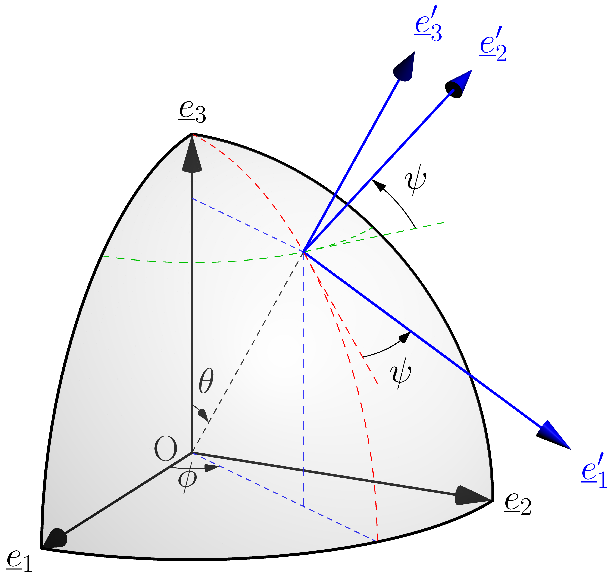
\includegraphics[width=0.4\textwidth,height=\textheight]{appendices/../images/sphcoor.pdf}

}

\caption{\label{fig-eurlerangles}Euler angles}

\end{figure}

The rotation of Eurler angles \((\theta,\phi,\psi)\) applies on a \(p\)
order tensor \(\mathcal{T}\) as
\begin{equation}\protect\hypertarget{eq-rotT}{}{
\mathcal{T}=
\mathcal{T}_{i_1,\ldots,i_p} \,\ve{i_1}\otimes\ldots\otimes\ve{i_{p}}
\overset{\uu{R}}{\longmapsto}
\uu{R}(\mathcal{T})=
\mathcal{T}_{i_1,\ldots,i_p} \,(\uu{R}\cdot\ve{i_1})\otimes\ldots\otimes(\uu{R}\cdot\ve{i_{p}})
}\label{eq-rotT}\end{equation}

The application of (\ref{eq-rotT}) to a second-order tensor \(\uu{a}\)
therefore gives \begin{equation}\protect\hypertarget{eq-rotT2}{}{
\uu{R}(\uu{a})=\uu{R}\cdot 
\uu{a}
\cdot\trans{\uu{R}}
}\label{eq-rotT2}\end{equation} and to a fourth-order tensor
\(\uuuu{T}\) \begin{equation}\protect\hypertarget{eq-rotT4}{}{
\uu{R}(\uuuu{T})=(\uu{R}\sboxtimes\uu{R}):
\uuuu{T}
:\trans{(\uu{R}\sboxtimes\uu{R})}
}\label{eq-rotT4}\end{equation} where the fourth-order rotation tensor
\(\uuuu{R}=\uu{R}\sboxtimes\uu{R}\) can be expressed in Kelvin-Mandel
notation (\ref{eq-KM4}) by means of the components of \(\uu{R}\) defined
in (\ref{eq-rot3}) \begin{equation}\protect\hypertarget{eq-rot6}{}{
\scriptsize
\Mat(\uuuu{R},\mathcal{B})=
   \left(
\begin{array}{cccccc}
R_{1 1}^{2} & R_{1 2}^{2} & R_{1 3}^{2} & \sqrt{2}  R_{1 2}  R_{1 3} & \sqrt{2}  R_{1 1}  R_{1 3} & \sqrt{2}  R_{1 1}  R_{1 2} \\
R_{2 1}^{2} & R_{2 2}^{2} & R_{2 3}^{2} & \sqrt{2}  R_{2 2}  R_{2 3} & \sqrt{2}  R_{2 1}  R_{2 3} & \sqrt{2}  R_{2 1}  R_{2 2} \\
R_{3 1}^{2} & R_{3 2}^{2} & R_{3 3}^{2} & \sqrt{2}  R_{3 2}  R_{3 3} & \sqrt{2}  R_{3 1}  R_{3 3} & \sqrt{2}  R_{3 1}  R_{3 2} \\
\sqrt{2}  R_{2 1}  R_{3 1} & \sqrt{2}  R_{2 2}  R_{3 2} & \sqrt{2}  R_{2 3}  R_{3 3} & R_{2 2}  R_{3 3} + R_{2 3}  R_{3 2} & R_{2 1}  R_{3 3} + R_{2 3}  R_{3 1} & R_{2 1}  R_{3 2} + R_{2 2}  R_{3 1} \\
\sqrt{2}  R_{1 1}  R_{3 1} & \sqrt{2}  R_{1 2}  R_{3 2} & \sqrt{2}  R_{1 3}  R_{3 3} & R_{1 2}  R_{3 3} + R_{1 3}  R_{3 2} & R_{1 1}  R_{3 3} + R_{1 3}  R_{3 1} & R_{1 1}  R_{3 2} + R_{1 2}  R_{3 1} \\
\sqrt{2}  R_{1 1}  R_{2 1} & \sqrt{2}  R_{1 2}  R_{2 2} & \sqrt{2}  R_{1 3}  R_{2 3} & R_{1 2}  R_{2 3} + R_{1 3}  R_{2 2} & R_{1 1}  R_{2 3} + R_{1 3}  R_{2 1} & R_{1 1}  R_{2 2} + R_{1 2}  R_{2 1} \\
\end{array}
\right)
}\label{eq-rot6}\end{equation} It results that (\ref{eq-rotT4}) can be
seen as a classical rotation operation involving matrix multiplications
in \(\R^6\).

\hypertarget{sec-ISO}{%
\section{Fourth-order isotropic tensors}\label{sec-ISO}}

This paragraph concerns fourth-order tensors operating over symmetrical
second-order tensors, which allows to impose that they satisfy the minor
symmetries (\(C_{jikl}=C_{ijlk}=C_{ijkl}\)). The identity operator is
given by \begin{equation}\protect\hypertarget{eq-tensI}{}{
\uuuu{I}=\uu{1}\sboxtimes\uu{1}=
\frac{\delta_{ik}\delta_{jl}+\delta_{il}\delta_{jk}}{2}\,\ve{i}\otimes\ve{j}\otimes\ve{k}\otimes\ve{l}
}\label{eq-tensI}\end{equation} of identity matrix in Kelvin-Mandel
convention \begin{equation}\protect\hypertarget{eq-matI}{}{
\small
\Mat(\uuuu{I},\mathcal{B})=
   \left(
   \begin{array}{ccc|ccc}
   1 & 0 & 0 & 0 & 0 & 0 \\
   0 & 1 & 0 & 0 & 0 & 0 \\
   0 & 0 & 1 & 0 & 0 & 0 \\
   \hline
   0 & 0 & 0 & 1 & 0 & 0 \\
   0 & 0 & 0 & 0 & 1 & 0 \\
   0 & 0 & 0 & 0 & 0 & 1 \\
   \end{array}
   \right)
}\label{eq-matI}\end{equation}

It is classically proven that any minor-symmetrical fourth-order tensor
invariant by rotation (\ref{eq-rotT4}) write as a linear combination on
the two projectors \(\uuuu{J}\) and \(\uuuu{K}\) which respectively
extract the spherical and deviatoric part of any symmetrical
second-order tensor \begin{equation}\protect\hypertarget{eq-JKext}{}{
\uuuu{J}:\uu{a}=\frac{1}{3}\tr{\uu{a}}\,\uu{1}
\quad \textrm{and} \quad
\uuuu{K}:\uu{a}=\uu{a}-\frac{1}{3}\tr{\uu{a}}\,\uu{1}
}\label{eq-JKext}\end{equation} In other words, \(\uuuu{J}\) and
\(\uuuu{K}\) are defined by
\begin{equation}\protect\hypertarget{eq-JK}{}{
\uuuu{J}=\frac{1}{3}\uu{1}\otimes\uu{1}
\quad \textrm{and} \quad
\uuuu{K}=\uuuu{I}-\uuuu{J}=\uu{1}\sboxtimes\uu{1}-\frac{1}{3}\uu{1}\otimes\uu{1}
}\label{eq-JK}\end{equation} their components by
\begin{equation}\protect\hypertarget{eq-JKijkl}{}{
J_{ijkl}=\frac{1}{3}\delta_{ij}\delta_{ik}
\quad \textrm{and} \quad
K_{ijkl}=\frac{\delta_{ik}\delta_{jl}+\delta_{il}\delta_{jk}}{2}-\frac{1}{3}\delta_{ij}\delta_{ik}
}\label{eq-JKijkl}\end{equation} and their matrices in Kelvin-Mandel
notation relatively to any orthonormal frame by
\begin{equation}\protect\hypertarget{eq-matJ}{}{
\small
\Mat(\uuuu{J},\mathcal{B})=
   \left(
   \begin{array}{ccc|ccc}
   \frac{1}{3} & \frac{1}{3} & \frac{1}{3} & 0 & 0 & 0 \\
   \frac{1}{3} & \frac{1}{3} & \frac{1}{3} & 0 & 0 & 0 \\
   \frac{1}{3} & \frac{1}{3} & \frac{1}{3} & 0 & 0 & 0 \\
   \hline
   0 & 0 & 0 & 0 & 0 & 0 \\
   0 & 0 & 0 & 0 & 0 & 0 \\
   0 & 0 & 0 & 0 & 0 & 0 \\
   \end{array}
   \right)
}\label{eq-matJ}\end{equation}

\begin{equation}\protect\hypertarget{eq-matK}{}{
\small
\Mat(\uuuu{K},\mathcal{B})=
   \left(
   \begin{array}{ccc|ccc}
   \frac{2}{3} & \frac{-1}{3} & \frac{-1}{3} & 0 & 0 & 0 \\
   \frac{-1}{3} & \frac{2}{3} & \frac{-1}{3} & 0 & 0 & 0 \\
   \frac{-1}{3} & \frac{-1}{3} & \frac{2}{3} & 0 & 0 & 0 \\
   \hline
   0 & 0 & 0 & 1 & 0 & 0 \\
   0 & 0 & 0 & 0 & 1 & 0 \\
   0 & 0 & 0 & 0 & 0 & 1 \\
   \end{array}
   \right)
}\label{eq-matK}\end{equation}

The following relationships are easily obtained
\begin{equation}\protect\hypertarget{eq-relJK}{}{
\uuuu{J}:\uuuu{J}=\uuuu{J}
\quad ; \quad
\uuuu{K}:\uuuu{K}=\uuuu{K}
\quad ; \quad
\uuuu{J}:\uuuu{K}=\uuuu{0}
\quad ; \quad
\uuuu{J}::\uuuu{J}=1
\quad ; \quad
\uuuu{K}::\uuuu{K}=5
}\label{eq-relJK}\end{equation}

The isotropisation of any fourth-order tensor \(\uuuu{T}\) is defined by
(\protect\hyperlink{ref-bornert2001a}{Bornert et al., 2001})
\begin{equation}\protect\hypertarget{eq-isoT}{}{
\ISO(\uuuu{T})=\left(\uuuu{T}::\uuuu{J}\right)\,\uuuu{J}+\left(\frac{\uuuu{T}::\uuuu{K}}{5}\right)\,\uuuu{K}
}\label{eq-isoT}\end{equation} It is easy to show that (\ref{eq-isoT})
is no other than the closest isotropic tensor to \(\uuuu{T}\) if the
distance is chosen as the euclidean one i.e.~associated to the scalar
product (\ref{eq-dot4}). Note however that this isotropisation relying
on euclidean distance to the set of isotropic tensors does not lead to
the same result if \(\uuuu{T}'\) is considered instead of \(\uuuu{T}\).
Other distance definitions such as log-Euclidean distance fullfilling
invariance by inversion are analyzed in
(\protect\hyperlink{ref-morin2020}{Morin et al., 2020}).

\hypertarget{sec-TI}{%
\section{Fourth-order transversely isotropic tensors and Walpole
basis}\label{sec-TI}}

The Walpole basis ((\protect\hyperlink{ref-walpole1984}{Walpole, 1984}),
(\protect\hyperlink{ref-brisard2014a}{Brisard, 2014})\footnote{see
  \url{https://sbrisard.github.io/posts/20140226-decomposition_of_transverse_isotropic_fourth-rank_tensors.html}})
allowing to write any fourth-order transversely isotropic relatively to
a an axis oriented by the unit vector \(\n\) is composed of the six
following tensors built from \(\uu{1}_n=\n\otimes\n\) and
\(\uu{1}_T=\uu{1}-\uu{1}_n\)
\begin{equation}\protect\hypertarget{eq-WalpoleBasis}{}{\begin{aligned}
& \uuuu{E}_1=\uu{1}_n\otimes\uu{1}_n
\quad\textrm{ ; }\quad
\uuuu{E}_2=\frac{\uu{1}_T\otimes\uu{1}_T}{2}
&\textrm{ ; }&
\uuuu{E}_3=\frac{\uu{1}_n\otimes\uu{1}_T}{\sqrt{2}}
\quad\textrm{ ; }\quad
\uuuu{E}_4=\frac{\uu{1}_T\otimes\uu{1}_n}{\sqrt{2}}
&(a) \\
& \uuuu{E}_5=\uu{1}_T\sboxtimes\uu{1}_T-\frac{\uu{1}_T\otimes\uu{1}_T}{2}
&\textrm{ ; }&
\uuuu{E}_6=\uu{1}_T\sboxtimes\uu{1}_n+\uu{1}_n\sboxtimes\uu{1}_T
&(b)
\end{aligned}}\label{eq-WalpoleBasis}\end{equation}

Any transversely isotropic fourth-order tensor can be decomposed as
\begin{equation}\protect\hypertarget{eq-decWalpole}{}{
{\uuuu{L}} = {\ell}_{1}\,{\uuuu{E}}_{1} + {\ell}_{2}\,{\uuuu{E}}_{2} +
{\ell}_{3}\,{\uuuu{E}}_{3}+ {\ell}_{4}\,{\uuuu{E}}_{4}+ {\ell}_{5}\,{\uuuu{E}}_{5}+
{\ell}_{6}\,{\uuuu{E}}_{6}
}\label{eq-decWalpole}\end{equation}

The six parameters can be conveniently gathered in a triplet composed of
a \(2 \times 2\) matrix containing the four first parameters \(\ell_i\)
(\(1\leq i \leq 4\)) and the two last parameters \(\ell_5\) and
\(\ell_6\) \begin{equation}\protect\hypertarget{eq-syntWalpole}{}{
\uuuu{L} \equiv \left( L , {\ell}_{5} , {\ell}_{6}
\right) , \quad
L = \left(
      \begin{array}{cc}
        {\ell}_{1} & {\ell}_{3} \\
        {\ell}_{4} & {\ell}_{2} \\
      \end{array}
    \right)
}\label{eq-syntWalpole}\end{equation}

Such a synthetic notation allows simple calculations of products and
inverses which consist in classical matrix or scalar products and
inverses
\begin{equation}\protect\hypertarget{eq-calWalpole}{}{\begin{aligned}
& \uuuu{L} : \uuuu{M} \equiv \left( L M , {\ell}_{5} m_5 , {\ell}_{6} m_6
\right)
&(a) \\
& {\uuuu{L}}^{-1} \equiv \left( {L}^{-1} , \frac{1}{{\ell}_{5}} , \frac{1}{{\ell}_{6}}
\right)
&(b)
\end{aligned}}\label{eq-calWalpole}\end{equation}

\hypertarget{sec-hill_elas}{%
\chapter{Hill polarization tensor in elasticity}\label{sec-hill_elas}}

This section recalls some results about the calculation of the Hill
polarization tensors related to a matrix of stiffness \(\mathbb{C}\) and
an ellipsoid \(\mathcal{E}_{\uu{A}}\) of equation \[
\uv{x}\in\mathcal{E}_{\uu{A}}
\quad\Leftrightarrow\quad
\uv{x}\cdot(\trans{\uu{A}}\cdot\uu{A})^{-1}\cdot\uv{x}\leq 1
\] where \(\uu{A}\) is an invertible second-order tensor so that
\(\trans{\uu{A}}\cdot\uu{A}\) is a positive definite symmetric tensor
associated to 3 radii (eigenvalues \(a\geq b \geq c\) possibly written
\(\rho_1 \geq \rho_2 \geq \rho_3\) for convenience) and 3 angles
(orientation of the frame of eigenvectors
\(\uv{e}_1, \uv{e}_2, \uv{e}_3\))
\begin{equation}\protect\hypertarget{eq-ellipsoid}{}{
\trans{\uu{A}}\cdot\uu{A}=a^2 \uv{e}_1\otimes\uv{e}_1 + b^2 \uv{e}_2\otimes\uv{e}_2 + c^2 \uv{e}_3\otimes\uv{e}_3 = \sum_{i=1}^3 \rho_i \uv{e}_i\otimes\uv{e}_i
}\label{eq-ellipsoid}\end{equation}

\hypertarget{general-expression}{%
\section{General expression}\label{general-expression}}

A general expression of the elastic polarization tensor is derived in
(\protect\hyperlink{ref-willis1977}{Willis, 1977}) (see also
(\protect\hyperlink{ref-mura1987}{Mura, 1987}))
\begin{equation}\protect\hypertarget{eq-Hill}{}{\begin{aligned}
\uuuu{P}(\uu{A},\uuuu{C})&=\frac{1}{4\pi}
\int_{\norm{\uv{\zeta}}=1}
(\uu{A}^{-1}\cdot\uv{\zeta})\sotimes
\Big((\uu{A}^{-1}\cdot\uv{\zeta})\cdot\uuuu{C}
\cdot(\uu{A}^{-1}\cdot\uv{\zeta})\Big)^{-1}
\sotimes(\uu{A}^{-1}\cdot\uv{\zeta})
\ud S_\zeta\\
&=
\frac{\det{\uu{A}}}{4\pi}
\int_{\norm{\uv{\xi}}=1}
\frac{\uv{\xi}\sotimes
(\uv{\xi}\cdot\uuuu{C}
\cdot\uv{\xi})^{-1}
\sotimes\uv{\xi}}{\norm{\uu{A}\cdot\uv{\xi}}^3}
\ud S_{\xi}
\end{aligned}}\label{eq-Hill}\end{equation}

When \(\uuuu{C}\) is arbitrarily anisotropic, it is necessary to resort
to numerical cubature to estimate \(\uuuu{P}\) as proposed in
(\protect\hyperlink{ref-ghahremani1977}{Ghahremani, 1977}),
(\protect\hyperlink{ref-gavazzi1990}{Gavazzi and Lagoudas, 1990}) or
(\protect\hyperlink{ref-masson2008}{Masson, 2008}). However in some
cases of anisotropy, analytical solutions are available
((\protect\hyperlink{ref-withers1989}{Withers, 1989}),
(\protect\hyperlink{ref-barthelemyIJES2020_hilltrans}{Barthélémy,
2020})). The case of isotropic matrix is particularly developed in the
next section.

\hypertarget{isotropic-matrix}{%
\section{Isotropic matrix}\label{isotropic-matrix}}

In this section, the matrix is assumed isotropic so that its stiffness
tensor writes by means of a bulk \(k\) and shear \(\mu\) or Lamé
\(\lambda\) and \(\mu\) moduli or even Young modulus \(E\) and Poisson
ratio \(\nu\) with \(k=\frac{E}{3(1-2\nu)}\) and
\(\mu=\frac{E}{2(1+\nu)}\).
\begin{equation}\protect\hypertarget{eq-isoC}{}{\begin{aligned}
\uuuu{C} =& {} 3k\uuuu{J}+2\mu\uuuu{K} =  3\lambda\uuuu{I}+2\mu\uuuu{K}\\
 & \quad\textrm{with}\quad J_{ijkl}=\frac{\delta_{ij}\delta_{kl}}{3},
I_{ijkl}=\frac{\delta_{ik}\delta_{jl}+\delta_{il}\delta_{jk}}{2}
\textrm{ and }
\uuuu{K}=\uuuu{I}-\uuuu{J}
\end{aligned}}\label{eq-isoC}\end{equation}

Introducing (\ref{eq-isoC}) in (\ref{eq-Hill}) leads to after some
algebra \[
\uuuu{P}=
\frac{1}{\lambda+2\,\mu}
\uuuu{U}
+\frac{1}{\mu}(\uuuu{V}-\uuuu{U})
\] where the tensors \(\uuuu{U}\) and \(\uuuu{V}\), depending only on
the ellipsoidal tensor \(\uu{A}\) of (\ref{eq-ellipsoid}), are given by
(see (\protect\hyperlink{ref-barthelemyIJES2020_hilltrans}{Barthélémy,
2020})) \[\begin{aligned}
\uuuu{U} &= \frac{\det{\uu{A}}}{4\pi}
\int_{\norm{\uv{\xi}}=1}
\frac{\uv{\xi}\otimes\uv{\xi}\otimes\uv{\xi}\otimes\uv{\xi}}
{\norm{\uu{A}\cdot\uv{\xi}}^3}\ud S_{\xi}\\
&=
\frac{1}{4\pi}
\int_{\norm{\uv{\zeta}}=1}
\frac{%
(\uu{A}^{-1}\cdot\uv{\zeta})
\otimes
(\uu{A}^{-1}\cdot\uv{\zeta})
\otimes
(\uu{A}^{-1}\cdot\uv{\zeta})
\otimes
(\uu{A}^{-1}\cdot\uv{\zeta})
}{\norm{\uu{A}^{-1}\cdot\uv{\zeta}}^4}
\ud S_{\zeta}
\end{aligned}\] and \[\begin{aligned}
\uuuu{V} &= \frac{\det{\uu{A}}}{4\pi}
\int_{\norm{\uv{\xi}}=1}
\frac{\uv{\xi}\sotimes\uu{1}\sotimes\uv{\xi}}
{\norm{\uu{A}\cdot\uv{\xi}}^3}\ud S_{\xi}\\
&=
\frac{1}{4\pi}
\int_{\norm{\uv{\zeta}}=1}
\frac{%
(\uu{A}^{-1}\cdot\uv{\zeta})
\sotimes
\uu{1}
\sotimes
(\uu{A}^{-1}\cdot\uv{\zeta})
}{\norm{\uu{A}^{-1}\cdot\uv{\zeta}}^2}
\ud S_{\zeta}
\end{aligned}\] For an arbitrary ellipsoid defined by
(\ref{eq-ellipsoid}), the components of \(\uuuu{U}\) and \(\uuuu{V}\)
write \[\begin{aligned}
U_{iiii}&=\frac{3(I_i-\rho_i^2I_{ii})}{2} 
\quad\forall\, i\in\{1,2,3\}\\
U_{iijj}=U_{ijij}=U_{ijji}&=\frac{I_j-\rho_i^2I_{ij}}{2} 
=\frac{I_i-\rho_j^2I_{ij}}{2}
\quad\forall\, i\neq j\in\{1,2,3\}
\end{aligned}\] and \[\begin{aligned}
V_{iiii}&=I_i\quad\forall\, i\in\{1,2,3\}\\
V_{ijij}=V_{ijji}&=\frac{I_i+I_j}{4}
\quad\forall\, i\neq j\in\{1,2,3\}
\end{aligned}\] where the coefficients \(I_i\) and \(I_{ij}\) are given
by (note that \(I_i\) and \(I_{ij}\) are adapted from those provided in
(\protect\hyperlink{ref-kellogg1929}{Kellogg, 1929}) and
(\protect\hyperlink{ref-eshelby1957}{Eshelby, 1957}): they differ by a
factor of \(4\pi/3\) for \(I_{ij}\) with \(i\neq j\) and by \(4\pi\) for
the others)

\begin{itemize}
\tightlist
\item
  if \(a > b > c\) \[\begin{aligned}
    I_1&=\frac{a\,b\,c}{(a^2-b^2)\sqrt{a^2-c^2}}\,
    \left({\cal F}-{\cal E}\right)\\
    I_3&=\frac{a\,b\,c}{(b^2-c^2)\sqrt{a^2-c^2}}\,
    \left(\frac{b\sqrt{a^2-c^2}}{a\,c}-
    {\cal E}\right)\\
    I_2&=1-I_1-I_3\\
    I_{ij}&=\frac{I_j-I_i}{\rho_i^2-\rho_j^2}\quad\forall\, i\neq j\in\{1,2,3\}\\
    I_{ii}&=\frac{1}{3}\left(
    \frac{1}{\rho_i^2}-
    \sum_{j\neq i}I_{ij} \right) 
    \quad\forall\, i\in\{1,2,3\}
    \end{aligned}\]\\
  where \({\cal F}={\cal F}(\theta,\kappa)\) and
  \({\cal E}={\cal E}(\theta,\kappa)\) are respectively the elliptic
  integrals of the first and second kinds (see
  (\protect\hyperlink{ref-abramowitz1972}{Abramowitz and Stegun, 1972}))
  of amplitude and parameter \[
    \theta=\arcsin{\sqrt{1-\frac{c^2}{a^2}}}
    \quad;\quad
    \kappa=\sqrt{\frac{a^2-b^2}{a^2-c^2}}
    \]
\item
  if \(a > b = c\) (prolate spheroid) \[\begin{aligned}
    I_2=I_3&=a\,
    \frac{a\sqrt{a^2-c^2}-c^2\,\arcosh{(a/c)}}
    {2\left(a^2-c^2\right)^{3/2}}\\
    I_1&=1-2\,I_3\\
    I_{1i}=I_{i1}&=\frac{I_i-I_1}{a^2-\rho_i^2}\quad
    \forall\, i\in\{2,3\}\\
    I_{ij}&=\frac{1}{4}
    \left(\frac{1}{c^2}-I_{31} \right) 
    \quad\forall\, i,j\in\{2,3\}\\
    I_{11}&=\frac{1}{3}
    \left(\frac{1}{a^2}-2\,I_{31} \right)
    \end{aligned}\]
\item
  if \(a = b > c\) (oblate spheroid) \[\begin{aligned}
    I_1=I_2&=c\,
    \frac{a^2\,\arccos{(c/a)}-c\sqrt{a^2-c^2}}
    {2\left(a^2-c^2\right)^{3/2}}\\
    I_3&=1-2\,I_1\\
    I_{3i}=I_{i3}&=\frac{I_3-I_i}{\rho_i^2-c^2}\quad
    \forall\, i\in\{1,2\}\\
    I_{ij}&=\frac{1}{4}
    \left(\frac{1}{a^2}-I_{31} \right) 
    \quad\forall\, i,j\in\{1,2\}\\
    I_{33}&=\frac{1}{3}
    \left(\frac{1}{c^2}-2\,I_{31} \right)
    \end{aligned}\]
\item
  if \(a = b = c\) (sphere) \[\begin{aligned}
    I_1=I_2=I_3&=\frac{1}{3}\\
    I_{ij}&=\frac{1}{5\,a^2}\quad\forall\, i,j\in\{1,2,3\}
    \end{aligned}\]
\end{itemize}

In this last case of spherical inclusion (\(\uu{A}=\uu{1}\)),
\(\uuuu{U}\) and \(\uuuu{V}\) are simply decomposed as \[
\uuuu{U}=\frac{1}{3}\uuuu{J}+\frac{2}{15}\uuuu{K}
\quad\textrm{ and }\quad
\uuuu{V}=\frac{1}{3}\uuuu{I}
\]

\hypertarget{case-of-cracks}{%
\section{Case of cracks}\label{case-of-cracks}}

The case of cracks corresponds to ellipsoids for which the smallest
radius is very small compared to the two others, in other words the
characteristic tensor \(\uu{A}\) (\ref{eq-ellipsoid}) can be written
here \[
\uu{A}=
\uv{\ell}\otimes\uv{\ell}+
\eta\,\uv{m}\otimes\uv{m}+
\omega\,\uv{n}\otimes\uv{n}
\quad\textrm{with}\quad
\eta=\frac{b}{a}
\quad\textrm{and}\quad
\omega=\frac{c}{a}
\]

\begin{figure}

{\centering 

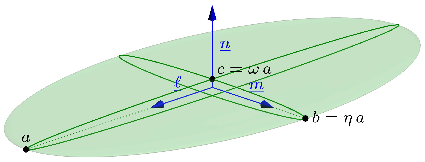
\includegraphics[width=0.7\textwidth,height=\textheight]{appendices/../images/crack.pdf}

}

\caption{\label{fig-crack}Ellipsoidal crack}

\end{figure}

In the case of cracks, it is useful to introduce the second Hill
polarization tensor defined as \[
\uuuu{Q}=\uuuu{C}-\uuuu{C}:\uuuu{P}:\uuuu{C}
\] and in particular \(\lim_{\omega\to 0}\omega\,\uuuu{Q}^{-1}\) in
which it is recalled that \(\uuuu{P}\) and thus \(\uuuu{Q}\) depend on
\(\omega\) such that the components
\(\left(\uuuu{Q}^{-1}\right)_{nijk}\) (with \(n\) corresponding to the
crack normal) behave as \(1/\omega\) when \(\omega\) tends towards
\(0\). The analytical expressions of this limit are fully detailed in
(\protect\hyperlink{ref-barthelemyIJES2021}{Barthélémy et al., 2021})
which recalls in particular that \(\uuuu{L}\) actually derives from a
symmetric second-order tensor \(\uu{B}\) as
\begin{equation}\protect\hypertarget{eq-L}{}{
\uuuu{L}=
\lim_{\omega\to 0} \omega\,\uuuu{Q}^{-1}
=\frac{3}{4}\,\uv{n}\sotimes\uu{B}\sotimes\uv{n}
}\label{eq-L}\end{equation}

For an arbitrarly anisotropic matrix, an algorithm allowing to estimate
the limit (\ref{eq-L}) is proposed in
(\protect\hyperlink{ref-barthelemyIJSS2009}{Barthélémy, 2009}) whereas
in the isotropic case \(\uu{B}\) writes \[
\uu{B}=
B_{nn}\,\uv{n}\otimes\uv{n}
+
B_{mm}\,\uv{m}\otimes\uv{m}
+
B_{\ell\ell}\,\uv{\ell}\otimes\uv{\ell}
\] with \[\begin{aligned}
B_{nn}&=\frac{8\,\eta\,(1-\nu^2)}{3\,E}\,
\frac{1}{\mathcal{E}_\eta}\label{eq:Bnn}\\
B_{mm}&=\frac{8\,\eta\,(1-\nu^2)}{3\,E}\,
\frac{1-\eta^2}{\left(1-(1-\nu)\,\eta^2\right)
\,\mathcal{E}_\eta-\nu\,\eta^2\,\mathcal{K}_\eta}\\
B_{\ell\ell}&=\frac{8\,\eta\,(1-\nu^2)}{3\,E}\,
\frac{1-\eta^2}{(1-\nu-\eta^2)\,\mathcal{E}_\eta+\nu\,\eta^2\,\mathcal{K}_\eta}
\end{aligned}\] where \(\mathcal{K}_\eta=\mathcal{K}(\sqrt{1-\eta^2})\)
and \(\mathcal{E}_\eta=\mathcal{E}(\sqrt{1-\eta^2})\) are the complete
elliptic integrals of respectively the first and second kind (see
(\protect\hyperlink{ref-abramowitz1972}{Abramowitz and Stegun, 1972})).
If the crack is circular, the components of \(\uu{B}\) become \[
B_{nn}=\frac{16\,(1-\nu^2)}{3\,\pi\,E}
\quad\textrm{;}\quad
B_{mm}=B_{\ell\ell}=\frac{B_{nn}}{1-\nu/2}
\]

\hypertarget{application-of-hill-calculation}{%
\section{Application of Hill
calculation}\label{application-of-hill-calculation}}

\hypertarget{definition-of-the-matrix-tensor}{%
\subsection{Definition of the matrix
tensor}\label{definition-of-the-matrix-tensor}}

\begin{Shaded}
\begin{Highlighting}[]
\NormalTok{C }\OperatorTok{=}\NormalTok{ stiff\_Enu(}\FloatTok{1.}\NormalTok{,}\FloatTok{0.2}\NormalTok{) }\OperatorTok{;} \BuiltInTok{print}\NormalTok{(C)}
\end{Highlighting}
\end{Shaded}

\begin{verbatim}
Order 4 ISO tensor | Param(size=2)=[ 1.66667 0.833333 ] | Angles(size=0)=[ ]
[ 1.11111 0.277778 0.277778 0 0 0 
  0.277778 1.11111 0.277778 0 0 0 
  0.277778 0.277778 1.11111 0 0 0 
  0 0 0 0.833333 0 0 
  0 0 0 0 0.833333 0 
  0 0 0 0 0 0.833333 ]
\end{verbatim}

\hypertarget{calculation-of-the-crack-compliance-uuuullim_omegato-0omegauuuuq-1}{%
\subsection{\texorpdfstring{Calculation of the crack compliance
\(\uuuu{L}=\lim_{\omega\to 0}\omega\,\uuuu{Q}^{-1}\)}{Calculation of the crack compliance \textbackslash uuuu\{L\}=\textbackslash lim\_\{\textbackslash omega\textbackslash to 0\}\textbackslash omega\textbackslash,\textbackslash uuuu\{Q\}\^{}\{-1\}}}\label{calculation-of-the-crack-compliance-uuuullim_omegato-0omegauuuuq-1}}

Note that in \emph{Echoes} it is necessary to provide an aspect ratio
\(\omega\) for the crack even if the crack compliance is actually
calculated as a limit (not depending on \(\omega\))

\begin{Shaded}
\begin{Highlighting}[]
\NormalTok{ω }\OperatorTok{=} \FloatTok{1.e{-}4}
\NormalTok{L }\OperatorTok{=}\NormalTok{ crack\_compliance(spheroidal(ω), C) }\OperatorTok{;} \BuiltInTok{print}\NormalTok{(L)}
\end{Highlighting}
\end{Shaded}

\begin{verbatim}
[[0.         0.         0.         0.         0.         0.        ]
 [0.         0.         0.         0.         0.         0.        ]
 [0.         0.         1.22230996 0.         0.         0.        ]
 [0.         0.         0.         0.67906109 0.         0.        ]
 [0.         0.         0.         0.         0.67906109 0.        ]
 [0.         0.         0.         0.         0.         0.        ]]
\end{verbatim}

\hypertarget{checking-the-aspect-ratio-for-which-omegauuuuq-1approx-lim_omegato-0omegauuuuq-1-is-acceptable}{%
\subsection{\texorpdfstring{Checking the aspect ratio for which
\(\omega\,\uuuu{Q}^{-1}\approx \lim_{\omega\to 0}\omega\,\uuuu{Q}^{-1}\)
is
acceptable}{Checking the aspect ratio for which \textbackslash omega\textbackslash,\textbackslash uuuu\{Q\}\^{}\{-1\}\textbackslash approx \textbackslash lim\_\{\textbackslash omega\textbackslash to 0\}\textbackslash omega\textbackslash,\textbackslash uuuu\{Q\}\^{}\{-1\} is acceptable}}\label{checking-the-aspect-ratio-for-which-omegauuuuq-1approx-lim_omegato-0omegauuuuq-1-is-acceptable}}

\begin{Shaded}
\begin{Highlighting}[]
\NormalTok{tω }\OperatorTok{=}\NormalTok{ np.logspace(}\OperatorTok{{-}}\DecValTok{5}\NormalTok{,}\DecValTok{1}\NormalTok{,}\DecValTok{20}\NormalTok{)}
\NormalTok{tabδ }\OperatorTok{=}\NormalTok{ []}
\ControlFlowTok{for}\NormalTok{ ω }\KeywordTok{in}\NormalTok{ tω:}
\NormalTok{    Q }\OperatorTok{=}\NormalTok{ hill\_dual(spheroidal(ω), C)}
\NormalTok{    Lω }\OperatorTok{=}\NormalTok{ ω}\OperatorTok{*}\NormalTok{np.linalg.inv(Q)}
\NormalTok{    δL }\OperatorTok{=}\NormalTok{ np.linalg.norm(Lω}\OperatorTok{{-}}\NormalTok{L)}\OperatorTok{/}\NormalTok{np.linalg.norm(L)}
\NormalTok{    tabδ.append(δL)}
\NormalTok{plt.figure(figsize}\OperatorTok{=}\NormalTok{(}\DecValTok{8}\NormalTok{,}\DecValTok{3}\NormalTok{))}
\NormalTok{plt.loglog(tω,tabδ,}\StringTok{\textquotesingle{}+{-}\textquotesingle{}}\NormalTok{)}
\NormalTok{plt.xlabel(}\VerbatimStringTok{r"$\textbackslash{}omega$"}\NormalTok{)}
\NormalTok{plt.ylabel(}\VerbatimStringTok{r"$\textbackslash{}frac\{||\textbackslash{}mathbb}\SpecialCharTok{\{L\}}\VerbatimStringTok{{-}\textbackslash{}omega\textbackslash{},\textbackslash{}mathbb}\SpecialCharTok{\{Q\}}\VerbatimStringTok{\^{}\{{-}1\}||\}\{||\textbackslash{}mathbb}\SpecialCharTok{\{L\}}\VerbatimStringTok{||\}$"}\NormalTok{)}
\NormalTok{plt.grid(}\VariableTok{True}\NormalTok{,which}\OperatorTok{=}\StringTok{\textquotesingle{}both\textquotesingle{}}\NormalTok{)}
\NormalTok{plt.show()}
\end{Highlighting}
\end{Shaded}

\begin{figure}[H]

{\centering 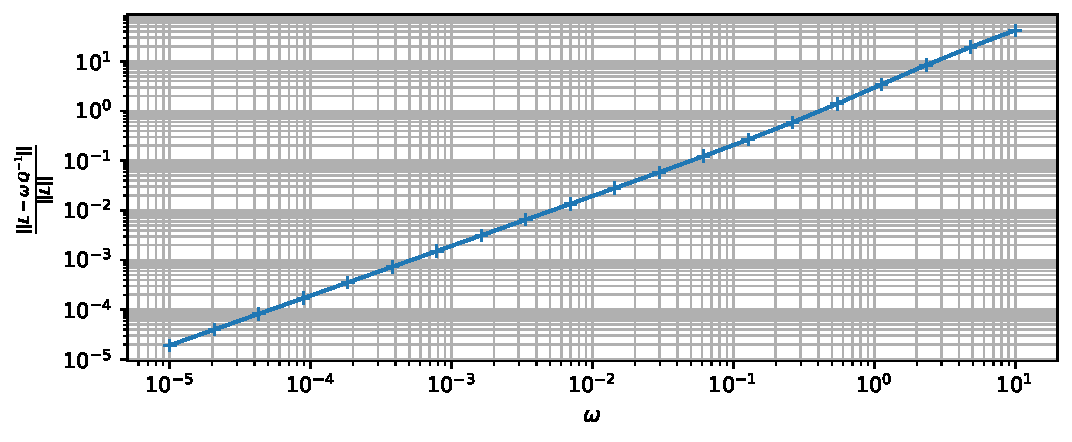
\includegraphics{appendices/hill_elas_files/figure-latex/fig-error-output-1.pdf}

}

\caption{\label{fig-error}Influence of the aspect ratio on the
contribution tensor}

\end{figure}

\hypertarget{sec-hill_cond}{%
\chapter{Hill polarization tensor in conductivity}\label{sec-hill_cond}}

\(\,\)



\end{document}
